\documentclass[11pt, a4paper, oneside]{article}
\usepackage{worksheet}
\usepackage{chessboard}

\begin{document}
	\author{L. Bung}
	\title{Vektorgeometrie: Einführung}
	\subject{Mathematik}
	\class{TG11}
	\maketitle
	
	\partnertask{Flugverbindungen zwischen Städten}
	
	Eine Fluggesellschaft plant eine neue Verbindung zwischen mehreren Städten in Deutschland.
	Um möglichst ökonomisch zu planen, sollen die Entfernungen und Richtungen zwischen den Städten berechnet werden.

	\begin{figure}[H]
		\centering
		\begin{tikzpicture}
			\node[anchor=south west] at (0,0) {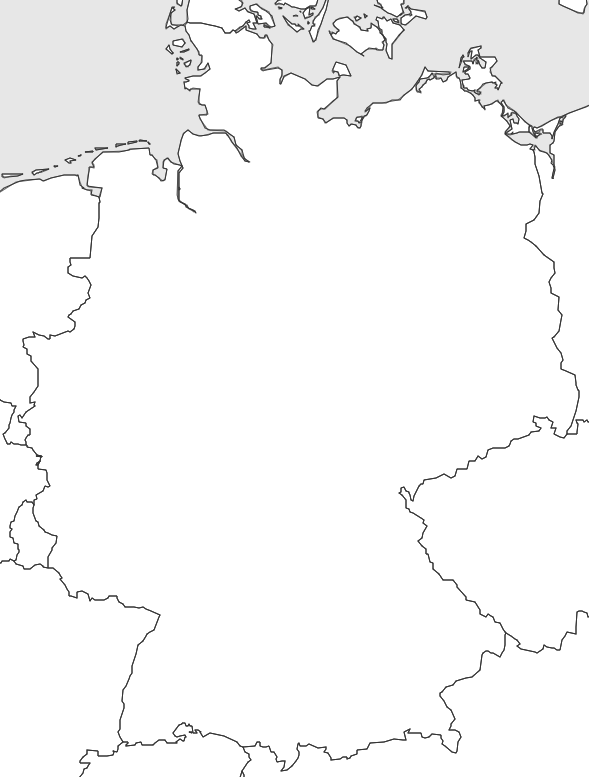
\includegraphics[width=.5\textwidth]{map_germany.png}};
			\draw[fill] (5.2,1.3) circle (1.5pt);
			\node[above, align=center] at (5.2,1.3) {München\\$(3|0)$};
			
			\draw[fill] (2.1,1.1) circle (1.5pt);
			\node[left=.3cm, align=center] at (2.1,1.1) {Freiburg\\$(0|0)$};
			
			\draw[fill] (6.6,7) circle (1.5pt);
			\node[above, align=center] at (6.6,7) {Berlin\\$(4.5|6)$};
			
			\draw[fill] (3,4) circle (1.5pt);
			\node[left, align=center] at (3,4) {Frankfurt\\$(1|3)$};
			
			\draw[fill] (3.6,6.9) circle (1.5pt);
			\node[left, align=center] at (3.6,6.9) {Hannover\\$(1.5|6)$};
			
			\node[left,fill=white] at (8,.25) {\tiny{\href{https://openstreetmap.org}{\copyright\ OpenStreetMap}}};
		\end{tikzpicture}
	\end{figure}
	a) Überlegen Sie sich eine Möglichkeit, dies mathematisch zu beschreiben.

	\checkered[4.5cm]
	
	\boxarea[10cm]
	
	b) Berechnen Sie die Verbindungsvektoren von Frankfurt zu den anderen vier Städten.
	
	\checkered[10cm]
	
	\partnertask{Springer im Schachspiel}
	
	Der Springer beim Schachspiel kann sich in jede Richtung wie ein ``L'' bewegen -- beispielweise ein Feld nach rechts und zwei Felder nach oben, oder zwei Felder nach links und ein Feld nach oben.
	
	\begin{minipage}{.49\textwidth}
		\centering
		\chessboard[hlabelformat=\arabic{ranklabel}, vlabelformat=\arabic{filelabel}, showmover=false, setwhite={Nd4}]
	\end{minipage}
	\hfill
	\begin{minipage}{.49\textwidth}
		\centering
		\chessboard[hlabelformat=\arabic{ranklabel}, vlabelformat=\arabic{filelabel}, showmover=false, setwhite={Nc6}]
	\end{minipage}

	a) Beschreiben Sie die möglichen Bewegungen der Springer mit Vektoren.
	Was fällt Ihnen beim Vergleich der beiden Situationen auf?

	\checkered[11cm]
	
	b) Überlegen Sie sich für die erste Situation, auf welchen Feldern der Springer im zweiten Zug landen kann.
	Wie könnten Sie das Resultat beiden Züge mithilfe der Vektoren aus Teilaufgabe a) darstellen?
	
	\checkered[10cm]
	
	\boxarea[10cm]
	
	\singletask{Lieferdrohne}
	
	Eine Lieferdrohne fliegt in einer Stadt, die als Koordinatensystem dargestellt wird.
	Die Startposition ist am Lagerhaus $L=(0|0)$.
	Nacheinander führt die Drohne folgende Lieferungen aus:
	
	\begin{enumerate}
		\item Die Drohne fliegt vom Lagerhaus zur ersten Lieferadresse und legt dabei die Bewegung $\vec{v_1} = \begin{pmatrix}4\\2\end{pmatrix}$ zurück.
		\item Als nächstes fliegt sie zur zweiten Adresse mit $\vec{v_2} = \begin{pmatrix}-1\\3\end{pmatrix}$.
		\item Zuletzt kehrt die Drohne zum Lager zurück.
	\end{enumerate}

	a) Bestimmen Sie die Gesamtbewegung der Drohne nach den ersten beiden Lieferungen.
	
	\checkered[6cm]
	
	b) Bestimmen Sie den Rückflugvektor zur Basis. Welche Eigenschaften muss dieser Vektor beim Vergleich mit dem in Teilaufgabe a) berechneten Vektor haben?
	
	\checkered[6cm]
	
	c) Zeichnen Sie den Flugweg der Drohne in ein Koordinatensystem ein.
	
	\checkered[10cm]
	
	d) Berechnen Sie die Gesamtlänge der geflogenen Strecke.
	
	\checkered[6cm]
\end{document}
